%KECReportFormat.tex
%%%%%%%%%%%%%%%%%%%%%%%%%%%%%%%%%%%%%%%%%%%%%%%%%%%%%%%%%%%%%%%%%%%%%%%%%%%
%DO NOT MAKE CHANGES IN THIS FILE

\documentclass[12pt, a4paper]{report}
\usepackage[left = 1.5in, right = 1in, top = 1in, bottom = 1in]{geometry}%for margin
\usepackage{amsfonts, amsmath, amssymb} %for mathematical equations
\usepackage{graphicx} %for images

\usepackage{times} %font Times New Roman Font
\usepackage{float} %required if you use H(strictly here) position for floats
\usepackage[skip = 8pt,tableposition=top, figureposition=bottom]{caption}%adjust spacing of captions and specify where captions are
\usepackage{hyperref} % for easy Navigation in document, also puts links in TOC, LOF, LOT...
\usepackage{setspace} %to change line spacing in some portion \singlespacing \onehalfspacing \doublespacing
\usepackage{acro} %for List of Abbrreviation and Symbol
\acsetup{first-style = short} % set to display only short form on the command \ac{}

%packages required for complex tables
\usepackage{bigstrut} 
\usepackage{multirow}
%package for greek letters
\usepackage[euler]{textgreek}
\renewcommand{\contentsname}{Table of Contents} %Change TOC Heading ... default is "Contents" 

\parindent 0pt	%removes the indent in paragraph
\setlength{\parskip}{18pt}	%for paragraph spacing
\renewcommand{\baselinestretch}{1.5}   %Line Spacing = 1.5 line-spaces

%to reduce spacing in sections
\usepackage{titlesec}
\titlespacing*{\section}{0pt}{0pt}{0pt} %left, top, bottom spacings
\titlespacing*{\subsection}{0pt}{0pt}{0pt}
\titlespacing*{\subsubsection}{0pt}{0pt}{0pt}
\titlespacing*{\paragraph}{0pt}{0pt}{0pt}
\titlespacing*{\subparagraph}{0pt}{0pt}{0pt}

%adjust fontsizes\ of sections
\titleformat*{\section}{\fontsize{14pt}{18pt}\bfseries}
\titleformat*{\subsection}{\fontsize{13pt}{18pt}\bfseries}
\titleformat*{\subsubsection}{\fontsize{12pt}{18pt}\bfseries}
\titleformat*{\paragraph}{\fontsize{12pt}{18pt}\bfseries}
\titleformat*{\subparagraph}{\fontsize{12pt}{18pt}\bfseries}

%to reduce separation between points in list
\usepackage{enumitem}
\setlist[enumerate]{nosep} % no separation between items in enumerate
\setlist[itemize]{nosep} % no separation between items in itemize
%use \vspace{-18pt} before list to reduce paragraph spacing between list and preceeding paragraph.

%Changes for Chapter Heading Spacing and formats for numbered chapters
\makeatletter
\def\@makechapterhead#1{%
  %\vspace*{50pt}%
  {  \MakeUppercase{\ifnum \c@secnumdepth >\m@ne
        \fontsize{16pt}{1}\bfseries \@chapapp \space \thechapter\vspace{5pt}\\
    \fi
    \interlinepenalty\@M
     \bfseries #1}\par\nobreak
    %\vskip 0pt
  }}
\makeatother

%%%%%%%%%%%%%%%%%%%%%%%%%%%%%%%%%%%%%%%%%%%%%%%%%%%%%%%%%%%
%to adjust Heading spacings and fonts For unnumbered chapters, TOC, LOF ...
\makeatletter
% Redefine the \chapter* header macro to remove vertical space
\def\@makeschapterhead#1{%
  %\vspace*{50\p@}% Remove the vertical space
  {\newpage \parindent \z@ \raggedright
    \normalfont
    \interlinepenalty\@M
    \center \fontsize{16pt}{1} \bfseries \MakeUppercase{#1}\par\nobreak
    %\vskip 18\p@ % adjust space after heading 18pt
  }}
\makeatother 
%%%%%%%%%%%%%%%%%%%%%%%%%%%%%%%%%%%%%%%%%%%%%%%%%%%%%%%%%%%

%%%%%%%%%%%%%%%%%%%%%%%%%%%%%%%%%%%%%%%%%%%%%%%%%%%%%%%%%%%%%%%%%%%%%%%%%%%
% newcommand for generating Cover Page
\newcommand{\KECcoverpage}
{
\begin{titlepage}
\begin{center}
\Large{\textbf{KANTIPUR ENGINEERING COLLEGE}}\\
\large{\textbf{(Affiliated to Tribhuvan University)}}\\
\large{\textbf{Dhapakhel, Lalitpur}}\\
\vfill	%vertically fill the space 
\begin{figure}[h] % h: put logo "here"
\begin{center}

\includegraphics[width=25mm, height = 25mm]{images/logo.png}
\end{center}
\end{figure}

\large{\textbf{[Subject Code: \subCode]}}\\ %Change This Line
\large{\textbf{A \MakeUppercase{\project} \MakeUppercase{\doc} ON}}\\ %Change This Line
\Large{\textbf{\MakeUppercase{\projectTitle}}}\\

\vfill	%vertically fill the space 
\large{\textbf{Submitted by:}}\\
\large{\textbf{\submittedBy}}\\
\vfill	%vertically fill the space 
\textbf{A \MakeUppercase{\project} SUBMITTED IN PARTIAL FULFILLMENT OF THE REQUIREMENT FOR THE DEGREE OF \MakeUppercase{\degree}}\\

\vfill	%vertically fill the space 
\large{\textbf{Submitted to:}}\\
\large{\textbf{\submittedTo}}\\
\vfill
\large{\textbf{\defMonth, \defYear}}
\pagebreak
\end{center}
\end{titlepage}
}
%%%%%%%%%%%%%%%%%%%%%%%%%%%%%%%%%%%%%%%%%%%%%%%%%%%%%%%%%%%%%%%%%%%%%%%
% newcommand for generating Cover Page
%Title Page
\newcommand{\KECtitlepage}
{
\begin{titlepage}
\begin{center}
\Large{\textbf{\MakeUppercase{\projectTitle}}}\\

\vfill	%vertically fill the space 

\large{\textbf{Submitted by:}}\\
\large{\textbf{\submittedBy}}\\

\if{\ne{\supervisor}{none}} \\ Displays Supervisor name only if it is not "none"
	\vfill	%vertically fill the space 
	\large{\textbf{Supervised by:}}\\
	\large{\textbf{\supervisor}}\\
	\large{\textbf{\degSup}}\\
\fi
\vfill	%vertically fill the space 
\textbf{A \MakeUppercase{\project} SUBMITTED IN PARTIAL FULFILLMENT OF THE REQUIREMENT FOR THE DEGREE OF \MakeUppercase{\degree}}\\

\vfill	%vertically fill the space 
\large{\textbf{Submitted to:}}\\
\large{\textbf{\submittedTo}}\\
\large{\textbf{Kantipur Engineering College}}\\
\large{\textbf{Dhapakhel, Lalitpur}}\\

\vfill
\large{\textbf{\defMonth, \defYear}}
\thispagestyle{empty}\\ %to remove page number
\pagebreak
\end{center}
\end{titlepage}
}
%%%%%%%%%%%%%%%%%%%%%%%%%%%%%%%%%%%%%%%%%%%%%%%%%%%%%%%%%%%%%%%%%%%%%%
%command for copyright page
\newcommand{\KECcopyright}
{
\chapter*{Copyright}%Required only for Final Defense of Major Project
\addcontentsline{toc}{chapter}{Copyright}
The author has agreed that the library, Kantipur Engineering Collage, may make this report freely available for inspection. Moreover the author has agreed that permission for extensive copying of this report for scholarly purpose may be granted by the supervisor(s), who supervised the project work recorded herein or, in their absence, by the Head of the Department wherein this project was done. It is understood that due recognition will be given to the author of this report and to the \submittedTo, Kantipur Engineering College in any use of the material of this report. Copying or publication or other use of this report for financial gain without approval of the \submittedTo, Kantipur Engineering College and author’s written permission is prohibited.\par Request for permission to copy or to make any other use of the material in this report in whole or in part should be addressed to:

Head\\
\submittedTo\\
Kantipur Engineering College\\
Dhapakhel, Lalitpur\\
Nepal
}
%%%%%%%%%%%%%%%%%%%%%%%%%%%%%%%%%%%%%%%%%%%%%%%%%%%%%%%%%%%%%%%%%%%%%%
%command for Approval Letter
\newcommand{\KECapproval}
{
\chapter*{Kantipur Engineering College
\vskip -10pt}%Required only for Final Defense of Major Project
\begin{center}
\fontsize{12.8pt}{1} %size decreaced to adjust department name in single line
\textbf{
\MakeUppercase{\submittedTo}\\ %for department name
}
\vskip 10pt
\fontsize{16pt}{1}
\textbf{APPROVAL LETTER}
\end{center}
\vskip -16pt
\addcontentsline{toc}{chapter}{Approval Letter}%
The undersigned certify that they have read and recommended to the Institute of Engineering for acceptance, a project report entitled "\projectTitle " submitted by \\
\submittedBy \\
in partial fulfillment for the degree of \degree. \par
{\vspace{25pt}
..........................................\\
Supervisor\\
\supervisor \\
\degSup\\
\vspace{25pt}\\
..........................................\\
External Examiner\\
\external\\
\degExternal\\
\vspace{25pt}\\
..........................................\\
\hod\\
Head of Department\\
\submittedTo
\vspace{10pt}\\
Date: \defMonth\space\defDay ,\space \defYear
\singlespacing\par
} %single spacing for the texts inside {}
}

%command for list of abbreviations
\newcommand{\KECloa}
{
%\chapter*{List of Abbreviations}
\addcontentsline{toc}{chapter}{List of Abbreviations}
\vskip -42pt % to reduce space due to invisivle acronym class name
{
\singlespacing
\printacronyms[include-classes=abbr, name= List of Abbreviations ]
}

}

%command for list of symbols
\newcommand{\KEClos}
{
\chapter*{List of Symbols}
\addcontentsline{toc}{chapter}{List of Symbols}
\vskip -42pt % to reduce space due to invisivle acronym class name{
{
\singlespacing
}
}

%command to adjust toc, lof, lot spacing
\newcommand{\KECadjusttocspacings}
{
\parskip 0pt % to remove paragraph spacing in TOC, LOF ...
\renewcommand{\baselinestretch}{0.1} % to adjust line spacing in toc
\newcommand*{\noaddvspace}{\renewcommand*{\addvspace}[1]{}}
\addtocontents{lof}{\protect\noaddvspace} %remove extra vertical space in LOF
\addtocontents{lot}{\protect\noaddvspace} %remove extra vertical space in LOT
}

 %includes the file KecReportFormat.tex that include all  necessary formattings

%%%%%%%%%%%%%%%%%%%%%%%%%%%%%%%%%%%%%%%%%%%%%%%%%%%%%%%%%%%%%%%%%%%%%%%%%%%
%Define Macros for Details of your Project
\newcommand{\project}{Minor Project } %Specify "Major Project" or "Minor Project"
\newcommand{\projectTitle}{SNAPTAG: CTRL+F FOR YOUR HANDWRITTEN NOTES} %specify "Title" of Your Project
\newcommand{\doc}{Final Report} % specify the document you are preparing eg. "Proposal", "Mid-Term Report" or "Final Report"32
% Note that You have to sibmit "Final Report" for Pre-final defense as well.
\newcommand{\subCode}{CT654} %specify Subject of Your Project
\newcommand{\degree}{Bachelor in Computer Engineering} %specify your degree
\newcommand{\submittedBy}%Specify Names and Roll/Symbol Numbers of the Project Group Members
{
%Edit Member Names and Roll/Symbol No. and adjust width (\makebox[width]) if necessary 
\makebox[10cm]{Ajaya Chaudhary \hfill [31056]}\\
\makebox[10cm]{Gaurav Giri \hfill [31078]}\\
\makebox[10cm]{Iza K.C. \hfill [31083]}\\
\makebox[10cm]{Lakesh Shrestha \hfill [31089]}
%\makebox[9cm]{Member Name \hfill [Roll/Symbol No.]}\\
} % Note that You must write your "Symbol Numbers"(Exam Roll Numbers) for Final Defenses

\newcommand{\submittedTo}{Department of Computer and Electronics Engineering} %specify your department
\newcommand{\hod}{Er. Rabindra Khati \\ Associate Professor}
 %specify Head ot the department
\newcommand{\defYear}{2024} %Defense Year
\newcommand{\defMonth}{Feb} %Defense Month- January, February, ...
\newcommand{\defDay}{} %specify Defense Day- 1, 2, ...

\newif\ifhassupervisor
\hassupervisorfalse % to display supervisor name use command- \hassupervisortrue
 
\newcommand{\supervisor}{Er. Bishal Thapa}
\newcommand{\degSup}{Project Coordinator\\ Department of Computer and Electronics Engineering}
\newcommand{\external}{External's Name}
\newcommand{\degExternal}{Designation of External\\Second line if required} %Specify Name of External for Major Project (Required for Black Book) , use multiple lines (\\) if necessary


%%%%%%%%%%%%%%%%%%%%%%%%%%%%%%%%%%%%%%%%%%%%%%%%%%%%%%%%%%%%%%%%%%%%%%%%%%%

%%%%%%%%%%%%%%%%%%%%%%%%%%%%%%%%%%%%%%%%%%%%%%%%%%%%%%%%%%%%%%%%%%%%%%%%%%%
%Define Abberviations and Symbols
% NOTE that Only those Abberviations and Symbols that are included in document(using command \ac{}) will be displayed in the List of Abberviations and Symbols.

%class 'abbr': for List of Abbreviations



%%%%%%%%%%%%%%%%%%%%%%%%%%%%%%%%%%%%%%%%%%%%%%%%%%%%%%%%%%%%%%%%%
% class `symbol': for List of Symbols
%\DeclareAcronym{transparencyFactor}{
%  short = \ensuremath{\alpha} ,
 % long  = Transparency Factor ,
 % sort  = Transparency Factor , % string to compare for sorting symbols... default string is the acronym name -"transparencyFactor"
  %class = symbol
%}% declares acronym named "transparencyFactor". Use \ac{UN} for short and \acl{UN} for long form.

%\DeclareAcronym{areaOfTriangle}{
 % short = \ensuremath{a} , % use \ensuremath{a} instead of $a$
 %% long  = Area of Triangle ,
 % sort  = Area of Triangle , % string to compare for sorting symbols
  %class = symbol
%}
%%%%%%%%%%%%%%%%%%%%%%%%%%%%%%%%%%%%%%%%%%%%%%%%%%%%%%%%%%%%%%%%%%%%%%%%%%%%%%%%%%%%%%%%%%%%%%%%%%%%

%The Document
\begin{document}

\KECcoverpage
\KECtitlepage

\pagenumbering{roman}
\KECapproval
\chapter*{Acknowledgment}
\addcontentsline{toc}{chapter}{Acknowledgment}%to include this chapter in TOC
We would like to express our gratitude to everyone who helped us to complete this project.
First and foremost, we would like to acknowledge the crucial role of our teachers of Department of Electronics and Computer Engineering for their guidance, support, and feedback throughout the project. Next, we would like
to give our gratitude to our classmates, for providing constructive feedback and engaging in
thought-provoking discussions regarding our project. Next, we’d like to thank all lecturers
of our department for guiding us through the beginning of our project to the end. Finally,
a special gratitude to our family and friends, for their love, encouragement, and support
throughout our academic journey.\\
Thank you all for your invaluable contributions to this project.\\
\makebox[10cm]{Ajaya Chaudhary \hfill }\\
\makebox[10cm]{Gaurav Giri \hfill }\\
\makebox[10cm]{Iza K.C. \hfill }\\
\makebox[10cm]{Lakesh Shrestha \hfill }
%to display members name under Acknowledgement
\chapter*{Abstract}
\addcontentsline{toc}{chapter}{Abstract}%to include this chapter in TOC 
SnapTag introduces an approach for efficiently analyzing handwritten documents by
leveraging image processing techniques and Named Entity Recognition (NER). The
primary objective is to develop a system capable of extracting meaningful information
from handwritten content provided by users and subsequently generating relevant tags for
improved document organization and categorization.\\\\
SnapTag employs image processing methods such as image binarization, thresholding,
denoising to enhance the quality of scanned handwritten documents. Through these
techniques, the system effectively preprocesses images, mitigating noise and improving
the clarity of handwritten text. Then, the methodology involves the integration of Canny
edge detection and Hough line transformation, coupled with K-means clustering, to
accurately detect document boundaries. Subsequent stages of the process incorporate
image segmentation to isolate words and characters, followed by a classification model
that identifies each character within the document. The character recognition phase utilizes a trained classification CNN model, to accurately
classify individual characters into predefined classes. This step is crucial for deciphering
the handwritten content and preparing it for further analysis.In the final stage, NER is
employed to extract meaningful tags from the processed document providing valuable
metadata that enhances the document's categorization and searchability.

{\textit{Keywords$-$Optical Character Recognition, Binarization, Thresholding, Denoising, Boundary Detection, Hough Line Transformation, K-Means Clustering, Convolutional Neural Network, Named Entity Recognition}} 

%{\par
%\begin{flushright}
%\vskip -20pt
%\setstretch{1.2}
%\submittedBy
%\end{flushright}}

%to adjust spacings for TOC, LOF, LOT
{

%TOC, LOF and LOT
\KECadjusttocspacings % defined in KECReportFormat.tex to adjust spacings
\makeatletter
% to add vskip of 18 point which is reduced when parskip is set to 0 in \LECadjustspacings
\def\@makeschapterhead#1{%
  %\vspace*{50\p@}% Remove the vertical space
  {\newpage \parindent \z@ \raggedright
    \normalfont
    \interlinepenalty\@M
    \center\fontsize{16pt}{1} \bfseries \MakeUppercase{#1}\par\nobreak
    \vskip 18\p@ % adjust space after heading 18pt
  }}
\makeatother 



\tableofcontents % prints table of contents
\listoffigures % prints list of figures
\addcontentsline{toc}{chapter}{List Of Figures}
%\listoftables % prints list of table
}
%%%%%%%%%%%%%%%%%%%%%%%%%%%%%%%%%%%%%%%%%%%%%%%%%%%%%%%%%%%%%%%%%%%%%%%%%%%

%comment this chapter if you don't have List of Abbreviations
%\KECloa % defined in KECReportFormat

%comment this chapter if you don't have List of Symbols
%\KEClos % defined in KECReportFormat


\chapter*{Abbreviations}
\addcontentsline{toc}{chapter}{Abbreviations}
\begin{tabbing}
\hspace{50mm}\=\kill
CNN \>  Convolutional Neural Network \\
EMNIST \> Extended Modified National Institute of Standards and Technology\\
NER \> Named Entity Recognition\\
OCR \> Optical Character Recognition\\
PDF \> Portable File Document\\
ReLU \> Rectified Linear Unit\\
% \DeclareAcronym{CNN}{
%  short = \ensuremath{a} , % use \ensuremath{a} instead of $a$
%  long  = Convolutional Neural Network,
%  sort  = Convolutional Neural Network, % string to compare for sorting symbols
%   class = symbol
% }
% \DeclareAcronym{EMNIST}{
%  short = \ensuremath{a} , % use \ensuremath{a} instead of $a$
%  long  = Extended Modified National Institute of Standards and Technology,
%  sort  = Extended Modified National Institute of Standards and Technology, % string to compare for sorting symbols
%   class = symbol
% }
\end{tabbing}
\newpage
\pagenumbering{arabic}

\chapter{Introduction}
\section{Background}\label{sec:bkgrnd}%label your section if you require to refer them somewhere else in your document.
When it comes to self-study or informal research, taking quick notes has long been a
favored practice. These notes serve as a valuable tool for reviewing and revisiting the
gathered information. Traditionally, pen and paper have been the preferred medium for
note-taking, as they offer a tangible and familiar experience. However, a common
challenge arises when these notes need to be quickly referenced or accessed for a
comprehensive overview.\\\\
Often, when we want to review the content of our notes, we may not have them readily
available. They might be left behind, misplaced, or simply inaccessible at the time we
need them. Additionally, the physical nature of pen and paper notes means that they are
not always well-preserved over an extended period. They can get lost, damaged, or suffer
from wear and tear, making them unreliable for long-term storage.\\\\
One approach to address the challenges of organizing and accessing handwritten notes is
to digitize them by storing them in the gallery or creating PDF documents. While this
offers convenience and preservation, it introduces its own set of issues. The unorganized
nature of storing notes as image files or PDFs makes it difficult to quickly locate specific
notes. Furthermore, the inability to easily search handwritten content within these digital
formats hinders efficient information retrieval. Existing OCR tools that enable searching
of handwritten text often come with premium access restrictions, creating a barrier for
users who desire a straightforward OCR solution without additional costs. Therefore,
there is a need for a free and unrestricted solution that provides efficient organization and
searching of handwritten notes, allowing users to easily access and retrieve information.
  
\section{Problem Statement}
The problem at hand is the lack of a free and unrestricted solution for organizing and
searching handwritten notes efficiently. The existing methods of storing notes in the
gallery or creating PDF documents offer convenience but lack proper organization and
search functionality. The handwritten content within these notes cannot be easily and
accurately searched using available tools, often requiring premium access for OCR
operations. This limitation hampers the ability of students and researchers to retrieve
specific information quickly and effectively.\\
The objective of the project is to develop a solution that addresses these issues by
providing a user-friendly platform for organizing handwritten notes and enabling efficient
keyword-based searching. This solution should be accessible, free of charge, and not
restricted by premium access limitations. By leveraging OCR technology, the project
aims to convert handwritten keywords within the notes into searchable digital text,
making it easier for users to retrieve relevant information when needed. Ultimately, this
project seeks to empower students and researchers by providing them with a convenient
and efficient tool for managing their handwritten notes and facilitating seamless
information retrieval.

\section{Objectives}
\begin{enumerate}[label=\roman*]
    \item To create a free and unrestricted platform for efficient organization and searching
    of handwritten notes, leveraging OCR technology to enable easy digitization and
    retrieval of information.
\end{enumerate}

\section{Application Scope}
 \begin{enumerate}
    \item This software can be utilized by researchers and academics to organize their
    handwritten research notes, allowing for efficient retrieval of information during
    the writing process. The OCR functionality enables quick keyword searching
    within the notes, helping researchers locate relevant information, references, and
    supporting evidence for their papers.
    \item Students can leverage the software to manage and organize their handwritten
    study notes, lecture summaries, and practice questions. The ability to search for
    keywords within the notes makes it easier for students to locate specific topics or
    concepts while preparing for exams.
    \item Language learners can utilize the software to organize their handwritten
    vocabulary lists, grammar rules, and language exercises. This enables them to
    access them quickly, helping in retention by facilitating vocabulary acquisition
    and language practice.
 \end{enumerate}
 \section{Features}
 \begin{enumerate}
    \item \textbf{Handwritten Note Digitization:}\\The platform allows users to easily convert their handwritten notes into digital
    format through scanning or capturing images, ensuring easy access and
    preservation.
    \item \textbf{Keyword-Based Searching:}\\Leveraging OCR technology, the platform enables users to search for specific
    keywords within their handwritten notes, providing quick and accurate retrieval of
    relevant information.
    \item \textbf{Cross Platform:}\\The platform can be accessed from various devices, such as computers, tablets,
    and smartphones, allowing users to retrieve their notes at any time.
    \item \textbf{Cost-Free and User-Friendly:}\\The platform is free to use and offers a user-friendly interface, ensuring that
    students and researchers can efficiently organize and search their handwritten
    notes without any financial barriers.
    \item \textbf{Efficient Content Indexing:}\\The platform automatically indexes the handwritten text within the notes,
    generating a searchable database of keywords. The indexing feature significantly
    improves the speed and accuracy of searching for specific information.
 \end{enumerate}
 \section{Feasibility Study}
 Before implementation of project design, the feasibility analysis of the project must be
done to move any further. The feasibility analysis of the project gives an idea on how the
project will perform and its impact in the real world scenario. So, it is of utmost
importance.
 \subsection{Economic Feasibility}
 Our system is economically achievable as a result of the development of several tools,
libraries, and frameworks. Since all the software required to construct it is free and
readily available online, this project is incredibly cost-effective. Only time and effort are
needed to create a worthwhile, genuinely passive system. The project doesn’t come at a
substantial cost. From an economic standpoint, the project appears successful in this
sense.
 \subsection{Technical Feasibility}
 The software needed to implement a project can be downloaded from a wide variety of
online resources. Technically speaking, the project is feasible as the necessary software is
easily available. We were able to learn the information we required for the project
through a variety of online sources, including classes. All the libraries and data are
accessible online for free because this project does not require any licensing costs. It is
technically possible if one has the necessary information and resources.
 \subsection{Operational Feasibility}
 Our project intends to improve hand-written notes taking experiences with a primary
focus on searching keywords in notes/documents to make it more accessible. The project
is intended for a sizable group of learners and students who desire to maintain their
handwritten notes. Consequently, our project is operationally feasible.
 \subsection{Schedule Feasibility}
 The workload of the project is divided amongst the project members. The scheduling is
 done according to an incremental model where different modules are planned to be
 assigned to the group members.So, the project fulfills the schedule feasibility
 requirements.
 %(GAntt chart here)
% \newpage
\begin{figure}[h]
    \centering
    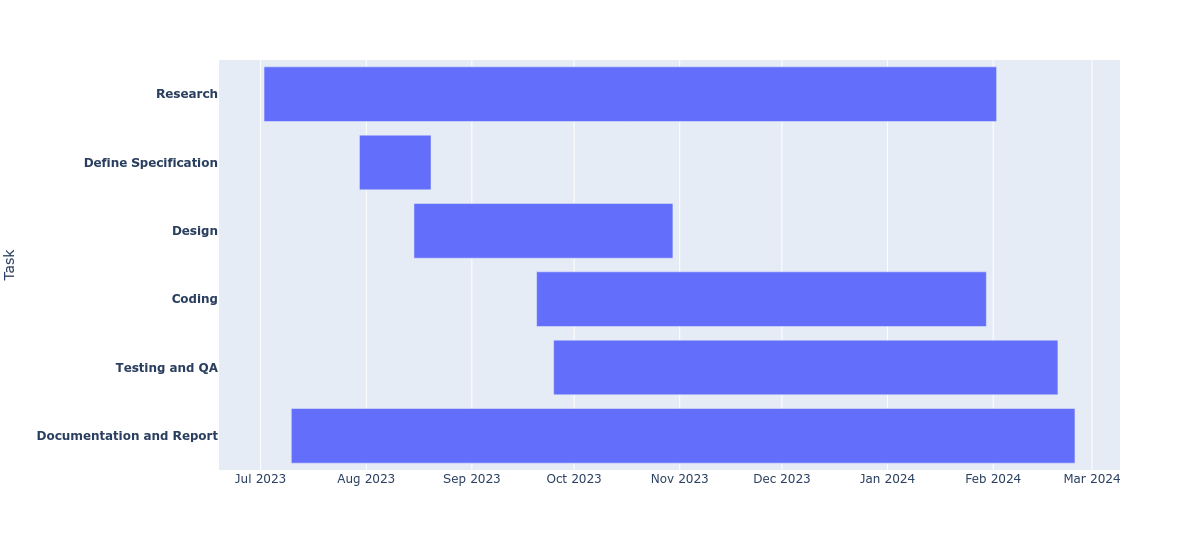
\includegraphics[scale=0.35]{images/GanttChart.png}
    \caption{Gantt Chart}\label{fig:my_label}
\end{figure}
\section{System Requirements}

\subsection{Development Requirements}
\begin{table}[h]
    \centering
    \caption{Development Requirements}
    \begin{tabular}{|l|l|}
        \hline
        \textbf{Software Requirements} & \textbf{Hardware Requirements}\\ \hline
        Programming Language: Python,Dart, Java & Camera: \(>\)= 12 Megapixels\\ \hline
        Design Tools: Figma & RAM: \(>\)= 8 GB\\ \hline
        OpenCV Library, spaCy & CPU: i5 10th (Recommended)\\ \hline
        Frameworks: Flutter, Tensorflow & GPU: P100\\ \hline
        Testing and Debugging Tools & Storage: \(>\)= 10 GB\\ \hline
    \end{tabular}
\end{table}
\newpage
\subsection{Deployment Requirements}
\begin{table}[ht]
    \centering
    \caption{Deployment Requirements}
    \begin{tabular}{|l|l|}
        \hline
        \textbf{Software Requirements} & \textbf{Hardware Requirements}\\ \hline
        Android: \(>\)= 10 & Camera: \(>\)= 12 Megapixels\\ \hline
        Read/Write FileSystem& RAM: \(>\) 4 GB\\ \hline
        Internet Accessibility & Storage: \(>\)= 5 GB\\ \hline
    \end{tabular}
\end{table}


\chapter{Literature Review}
Regardless of whether they are documented or not, every project has helped to shape the world as it is today.
Other researchers can benefit from documented projects by learning specifics about problems and how to solve
them. Additionally, they boostproject efficiency by removing the need to start the project from the beginning 
and specifying the starting point.
\section{Related Research}
S. Abbas et all introduced an intelligent and efficient handwritten script recognition system using deep
convolutional neural networks (CNNs). The research addresses several challenges in handwritten character 
recognition, such as distorted shapes, varying writing styles, and curved characters. To overcome these
issues, the proposed method incorporates extensive image processing and pattern recognition techniques.
The research utilizes a large dataset of 65,000 handwritten characters’ images for training and testing
the CNN model. The deep convolutional neural network, consisting of multiple hidden layers with numerous 
neurons, is trained on this dataset to recognize handwritten scripts. The system also employs three 
segmentation algorithms: line-based, word-based, and character-based, to accurately separate characters 
in the script before recognition. The results show promising accuracy of 90\% in recognizing handwritten 
scripts and effectively converting them into electronic text documents\cite{ghazal2022convolutional}.\\

D.V. Tropin et all present  a thorough investigation into the challenging problem of quadrilateral detection in computer vision tasks. The detection of quadrilaterals is a crucial step in various applications, including document processing, signboards, whiteboards, license plates, and more.The paper provides an overview of existing approaches to quadrilateral detection, including contour-based, region-based, and vertex-based methods. It  highlights the limitations and challenges faced by each approach, such as difficulties in handling occlusions, low contrast, strong lines, blurred images, and lack of a priori 
information about object structure. To address the limitations of existing methods, the paper introduces a novel combination of contour and region-based approaches. The main idea is to rank competing contour hypotheses based on the contrast between areas inside and outside the border. By leveraging both approaches in the quadrilateral scoring process, the authors report a 40\% decrease in ranking errors\cite{tropin2021approach}.\\

A. Tam et all introduced a novel system for automatically detecting signboards and extracting text from them, specifically tailored for guiding the navigation of autonomous robots indoors and outdoors. Unlike previous approaches, the system is not restricted to traffic signs and car plates; instead, it aims to detect a wide range of signboards, accommodating variations in shape, rotation, and scaling. The authors employ the Hough transform and other advanced processing schemes to achieve their goal. The system primarily focuses on identifying quadrilateral signboards present in images, assuming the entire signboard is visible and avoiding detection of overly small signboards with limited recognizability. To enhance text extraction accuracy, a geometric transformation is proposed to convert the detected quadrilaterals into rectangular shapes. The paper also discusses the segmentation of text from the found signboards. While the approach shows great promise, providing more extensive experimental evaluations and detailed discussions of segmentation techniques would further strengthen the paper's impact\cite{tam2003quadrilateral}. \\

G. Cohen et all present the significance of good benchmarks and standardized problems in machine learning and computer vision, particularly in the context of rapid advancements in these fields. It emphasizes the need for diverse benchmark tasks to comprehensively evaluate learning approaches and techniques. The authors introduce a suite of datasets called Extended Modified NIST (EMNIST) derived from the NIST Special Database 19, with the intention of providing a more challenging classification task for neural networks and learning systems. The datasets are designed to be drop-in replacements for existing systems, aligning with the image specifications and file formats of the well-known MNIST dataset. The paper thoroughly documents the dataset conversion process and presents benchmark results to validate the datasets. However, it acknowledges that MNIST, though widely used, may have lost its relevance as a challenging benchmark due 
to exceptionally high accuracies achieved by deep learning models, questioning the labeling integrity of the dataset. In contrast, the EMNIST datasets offer a more complex task that ensures the longevity of meaningful benchmarks in the field\cite{cohen2017emnist}.
\\
The Hough Line Transformation is a powerful image processing technique that has found widespread application in computer vision, image analysis, and pattern recognition. Proposed by Paul Hough in 1962, this method was initially designed for detecting straight lines in binary images, providing a robust solution to overcome the limitations of edge-based approaches. Over the years, researchers have extended and refined the Hough Line Transformation, making it a fundamental tool in computer vision for detecting and characterizing linear features in images. The Hough technique is particularly useful for computing a global description of features where the number of solution classes need not be known prior, given (possibly noisy) local measurements. The motivating idea behind the Hough technique for line detection is that each input measurement (e.g. coordinate point) indicates its contribution to a globally consistent solution (e.g. the physical line which gave rise to that image point)\cite{Ballard1982ComputerVision}. 

\chapter{Methodology}
\section*{}
\begin{figure}[h]
    \centering
        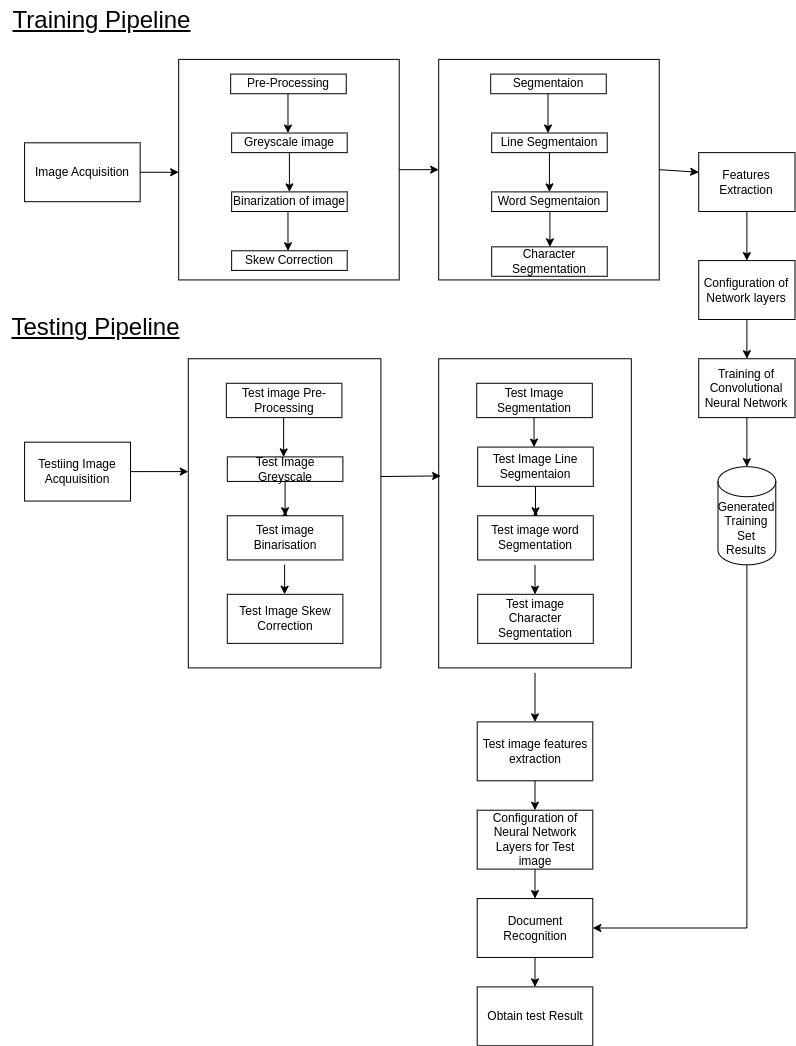
\includegraphics[scale=0.46]{images/Methodology.png}
        \caption{Block diagram for the working mechanism of the system}%\label{fig:fig1}
    \end{figure}
\newpage
\section{Working Mechanism}
The methodology diagram is shown above fig no. 3.1 which consists of several stages such as image acquisition i.e.testing image, pre-processing (grayscale conversion, binarization, document detection), segmentation (lines, words, and characters), feature extraction, and classification using CNN layers into\cite{Ishfar2020DocumentDetection} character classes.
\subsection{Image Acquisition}
The first step is to obtain a handwritten script through  scanning physical documentation or images using a camera.
\subsection{Pre-processing}
It is essential to enhance the quality and prepare the image for further analysis. This step includes Grayscale Conversion, Binarization, Noise Removal and skew correction. Grayscale conversion is used to reduce complexity of handling multiple color channels ( 24-bit to 8-bit). Binarization is used to convert grayscale images into black and white to make it easier for segmentation.\newline
Noise removal is used to remove unwanted variations in pixel intensity that degrade image quality. The proposed method uses a median filter to efficiently remove salt and pepper noise. This filter sorts adjacent pixel values and replaces the current pixel value with the median, reducing the noise and improving image.
\subsection{Document Detection}
The document detection is used for auto-cropping the image and correcting the perspective angle of the page of interest. For that quadrilateral points are obtained through the merged process of canny edge detection and hough transformation then KMeans Clustering that clusters the intersection points into 4 groups which are the quadrilaterals. Then through the quadrilaterals, perspective transformation is performed to get a good perspective of the page\cite{Ishfar2020DocumentDetection}.
\subsection{Segmentation}
In the segmentation process, we first tackle Line Segmentation, where the input image is       analyzed to identify lines of text. By finding dark centroids in the image, we can mark the positions of each line. We employ a projection profile-based algorithm for this task and address the issue of skewed text by applying skew correction techniques.\newline 
Moving on to Word Segmentation, our approach involves morphological dilation, which allows us to connect individual characters in a line, ultimately helping us to extract separate words. Using labeling techniques, we efficiently isolate and extract words from the connected components.\newline 
Character Segmentation is a crucial step, particularly for cursive handwriting. To address the challenges of cursive characters, we implement skeletonization and vertical projection techniques to detect potential segmentation points. A distance-based approach is utilized to avoid over-segmentation, ensuring that characters like 'm', 'n', 'u', 'v', 'w', etc., are correctly identified. For untouched characters, a vertical projection is employed to identify spaces between characters, facilitating their separation.\newline
Through these segmentation processes, we break down the handwriting image into lines, words, and individual characters, which is essential for accurate and efficient handwriting recognition.
\subsection{Features Extraction}
Feature extraction involves identifying important image features and saving them for further processing. It bridges the gap between pictorial and data representation in image processing. The proposed method employs a Convolutional Neural Network (CNN) for effective feature extraction, making the process more efficient and accurate.
\subsubsection{Training of Convolutional Neural Network}
The configured layers of Convolution Neural Network are shown below. To train the neural network, the dataset is divided into two sets: the training data and the testing data. The complex handwritten character dataset has data format of 28x28 ".png" format picture. The data set has a total of 62 categories of 0-9, a-z and A-Z, corresponding to the files "0" to "61" in the order of "label.txt". The data set is divided into two parts, the unprocessed original data image is stored in the "0" to "61" in the "V0.3/data" folder, and the binarized data image Stored in "0" to "61" in the "V0.3/data-bin" folder\cite{Ishfar2020DocumentDetection}.
\begin{figure}[h]
    \centering
        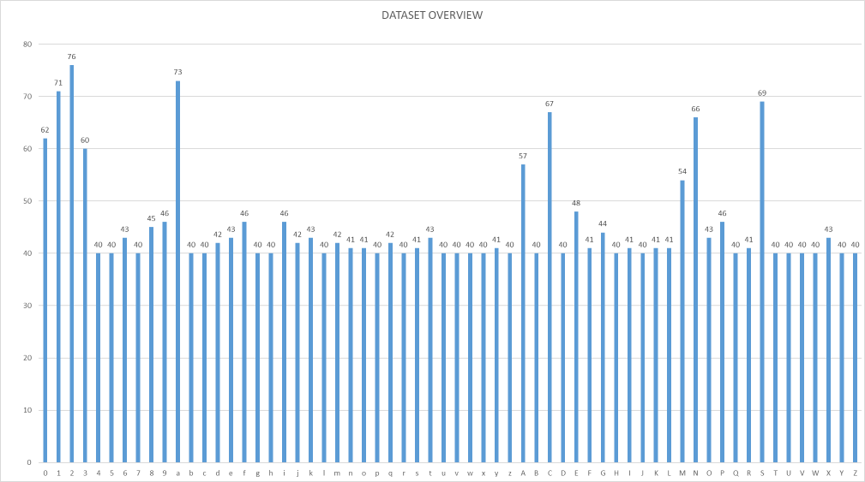
\includegraphics[scale=0.45]{images/Data_overview.png}
        \caption{Dataset overview for the A good CHoiCe}%\label{fig:fig1}
    \end{figure}
    The EMNIST also has 62 character classes divided into digit classes and letter classes containing a total 814,255 samples\cite{Ishfar2020DocumentDetection}.
    \begin{figure}[h]

        \centering
            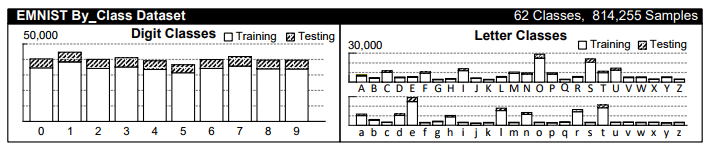
\includegraphics[scale=0.45]{images/EMNIST_Dataset.png}
            \caption{Visual representation of E MNIST dataset}%\label{fig:fig1}
        \end{figure}  
    \begin{figure}[h!]
        \centering
            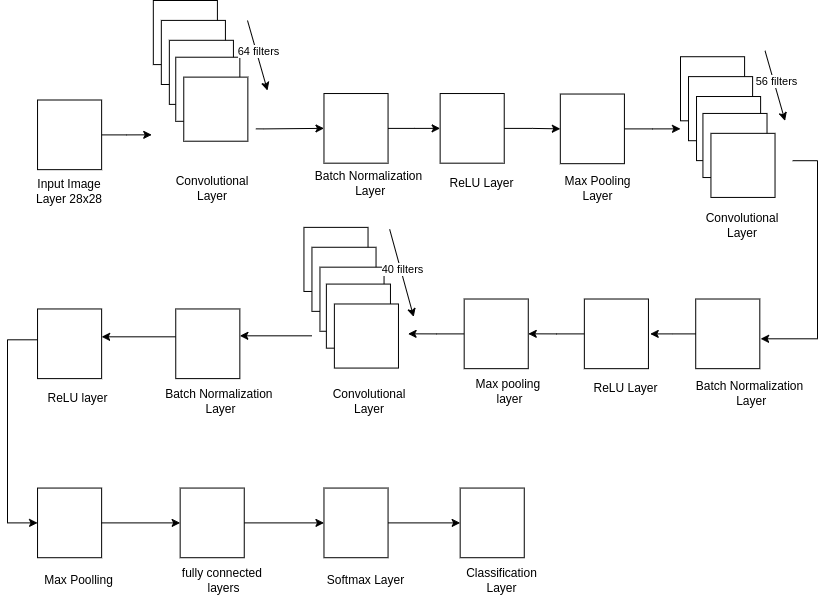
\includegraphics[scale=0.45]{images/CNN_model.png}
            \caption{Configured layers of Convolution Neural Network}%\label{fig:fig1}
        \end{figure} 
    \newpage
\newpage
\subsubsection{Document Recognition} 
The neural network used for image recognition involves four primary operations: Convolution, Non-Linearity (ReLU), Pooling, and Fully Connected Layer.
\begin{enumerate}
    
    \item Convolution: The convolution operation extracts features from the input image M using a filter matrix N. The resulting feature map \( f_{\text{con}}(k,l)\) can be calculated as follows:
    \begin{eqnarray}
        f_{\text{con}} = \text{convolution}(m,n) 
    \end{eqnarray}
     \begin{eqnarray}
         (m\bigotimes n)(k,l) = \sum_{m} \sum_{n}    M(m,n)  N(k-m,l-n) \quad
     \end{eqnarray}   
        
    
    
    
    \item Non-Linearity (ReLU): The ReLU function is applied element-wise to the feature map to introduce non-linearity and obtain the rectified feature map frec(xk): 
    \begin{eqnarray}
    f_{\text{Rec}} = \text{ReLU}(x,l) = \max(0, x_k)  \quad
    \end{eqnarray}   

    \item Pooling: Pooling reduces feature map dimensionality while preserving important information. The Max pooling technique selects the maximum value from a defined spatial matrix (e.g. 2x2):
    \begin{eqnarray}
    f_{\text{pool}}(k,l) = \max(x_k)
    \end{eqnarray}   

    \item Fully Connected Layer: In this layer, all neurons are connected to each other, and the output is used for classification.\newline
    Finally, the Softmax Layer outputs probabilities for each class of the handwritten characters. The Softmax function calculates the probability for an input element xk. belonging to label i as follows:
    \begin{eqnarray}
        p(O_i) = \text{softmax}(x_k) = \frac{\exp(x_k)}{\sum_{g = 1}^{y}   \exp(x_k)} 
    \end{eqnarray}
    
    The Classification Layer then identifies the recognized character based on the highest probability assigned by the Softmax Layer.
\end{enumerate}
\subsection{Named Entity Extraction using spaCy}
NER is a process in which anything that is denoted by a proper name or tag,for example, a location, an organization, or a person is identified as an entity.Named entities include things like geographical location, date, time, or money, and customization of the NER model for user-defined named entities is also possible\cite{shelar2020named}.\newline
spaCy is a free, open source library that allows advanced Natural Language Processing in Python. This library will be used to extract the unique word which will be used as tags for the image while searching it. Unique words are generated through named entity recognition for which "en\_core\_web\_sm" is used, which is a linguistic model.\newline
\section{Algorithm Used}
\begin{itemize}
    \item \textbf{Line Segmentation:} The Line Segmentation algorithm starts with image padding to avoid segmentation errors. It computes the horizontal projection to identify text regions and detects dark lanes using a threshold in the binary image. The algorithm labels and counts dark regions to determine total lines of text. Centroids are calculated for precise positioning and stored for further processing. x and y coordinates of centroids are extracted. Text regions are cropped based on consecutive y-coordinates for accurate segmentation, enabling proper division of each handwritten script line for improved recognition and analysis.
    \item \textbf{Word Segmentation:} The Word Segmentation algorithm aims to extract individual words from previously segmented lines of handwritten text. It involves three steps: first, dilating the line image to expand the pixels and enhance visual distinction between connected components; second, labeling the connected components to identify distinct words; and finally, separating the labeled components to obtain individual images of each word. These separated images represent the segmented words of the handwritten text.
    \item \textbf{Cursive Character Segmentation:} The Cursive Character Segmentation algorithm separates connected characters in a handwritten text image by skeletonizing the image and computing its vertical projection. It marks segmentation points using the "Segmentation Points" (SP) array, starting from the first character. For each column and row, it checks if certain conditions are met to identify connected characters. If these conditions are fulfilled, the algorithm stores the column in the SP array based on a threshold distance. After marking the segmentation points, it draws red lines on the word image for visualization and stores 0 in the rows of SP to disconnect the characters. This process paves the way for further character segmentation and recognition.
    \item \textbf{Untouched Character Segmentation:} The Untouched Character Segmentation algorithm effectively segments individual characters in a handwritten text image that have not been separated previously. It begins by padding the image for better segmentation and computes the Vertical Projection (VP) to identify character zones. Applying a threshold to the binary image detects dark lanes between letters. Each dark region is labeled, and the total character count is determined. Centroids are calculated for precise character positioning, and their x and y coordinates are extracted. The algorithm then crops text regions assuming a line between consecutive x-coordinates, ensuring accurate character segmentation. Cropped regions are stored separately, facilitating proper segmentation for s subsequent recognition and analysis.
  \end{itemize}
  \newpage
\section{System Diagrams}
The usecase diagram and activity diagram for SNAPTAG are given below:
\begin{figure}[h!]
    \centering
        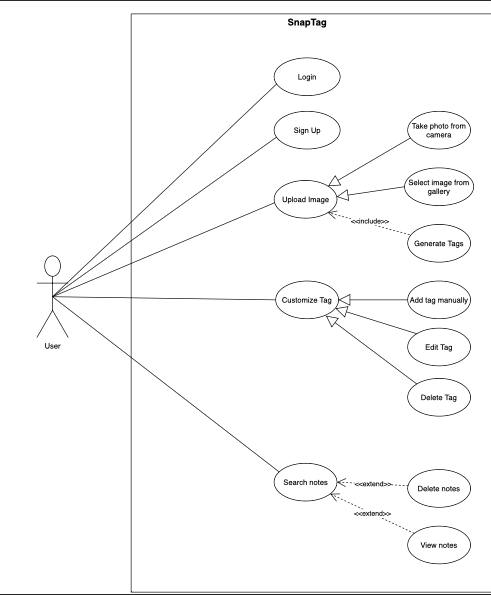
\includegraphics[scale=0.7]{output/usecase.png}
        \caption{UseCase Diagram}%\label{fig:fig1}
    \end{figure}
\newpage
\begin{figure}[h!]
     \centering
        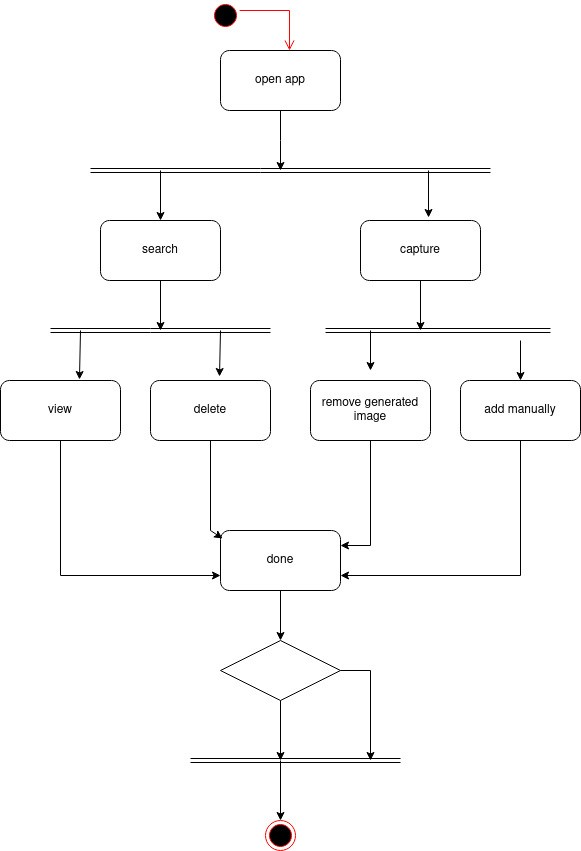
\includegraphics[scale=0.7]{output/activity.jpg}
        \caption{Activity Diagram}%\label{fig:fig1}
     \end{figure}
     \newpage
\newpage
\section{Software Development Model}
This project is developed using an incremental methodology since it offers a functioning prototype at an early stage of development. The requirements and scope of the project can be altered as necessary by studying the prototype. The rationale for the preference for this software development strategy is the flexibility offered by adopting the incremental technique. In this paradigm, the project goes through several releases or iterations prior to its official release.
\begin{figure}[h!]
    % \centering
        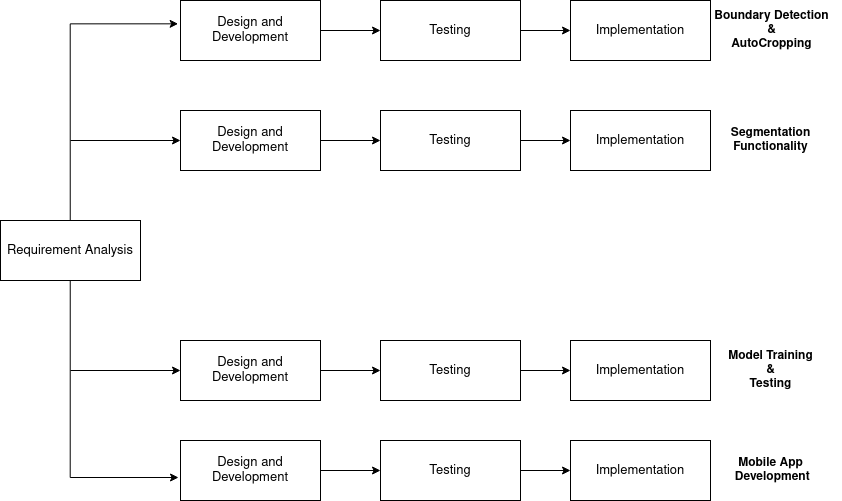
\includegraphics[scale=0.45]{images/SDLC.png}
        \caption{Incremental Model for development of SnapTag}%\label{fig:fig1}
    \end{figure}
\newpage
\chapter{Result And Discussion}
%\addcontentsline{toc}{chapter}{Result And Discussion}
\section{Result}
We have completed the design and development of the system along with the required output of the project. The project currently allows user to register and log-in into the system. User can post queries, answer, vote, follow other users and search queries.  Trending section shows most relevant post using half life decay algorithm.
\section{Work Done}
\begin{enumerate}
    \item Preprocessing: Common processing steps like Thresholding, De-noising, Resizing were done. In threshold, we used Otsu's Binarization due to its automatic optimal threshold value determination and avoiding having to choose a value. In order to do so, the cv2.threshold() function was used. Processing high resolution images are quite resource intensive. So, images were scaled down for faster processing using cv2.resize() function. And we performed de-noising to remove noise from images. To do this, we used cv2.fastNlMeansDenoising() function because of its faster processing while maintaining the denoising performance.
    \item Opening and closing: Opening and Closing are used as morphological operations to manipulate the shapes and structures of objects within an image. Closing and opening was used to improve the quality of the input image for further process of edge detection by reducing noise,smoothing contours . 
    \item Hough line transformation: Hough transformation was used after using Canny edge detection as this edge description is commonly obtained using Canny may be noisy, i.e. it may contain multiple edge fragments corresponding to a single whole feature. Furthermore, the output of an edge detector like Canny defines only where features are in an image, the work of the Hough transform is to determine both what the features are and how many of them exist in the image. 
    \newpage
    \newpage
    \begin{figure}[h]
        \centering
        \begin{minipage}[b]{0.30\linewidth}
            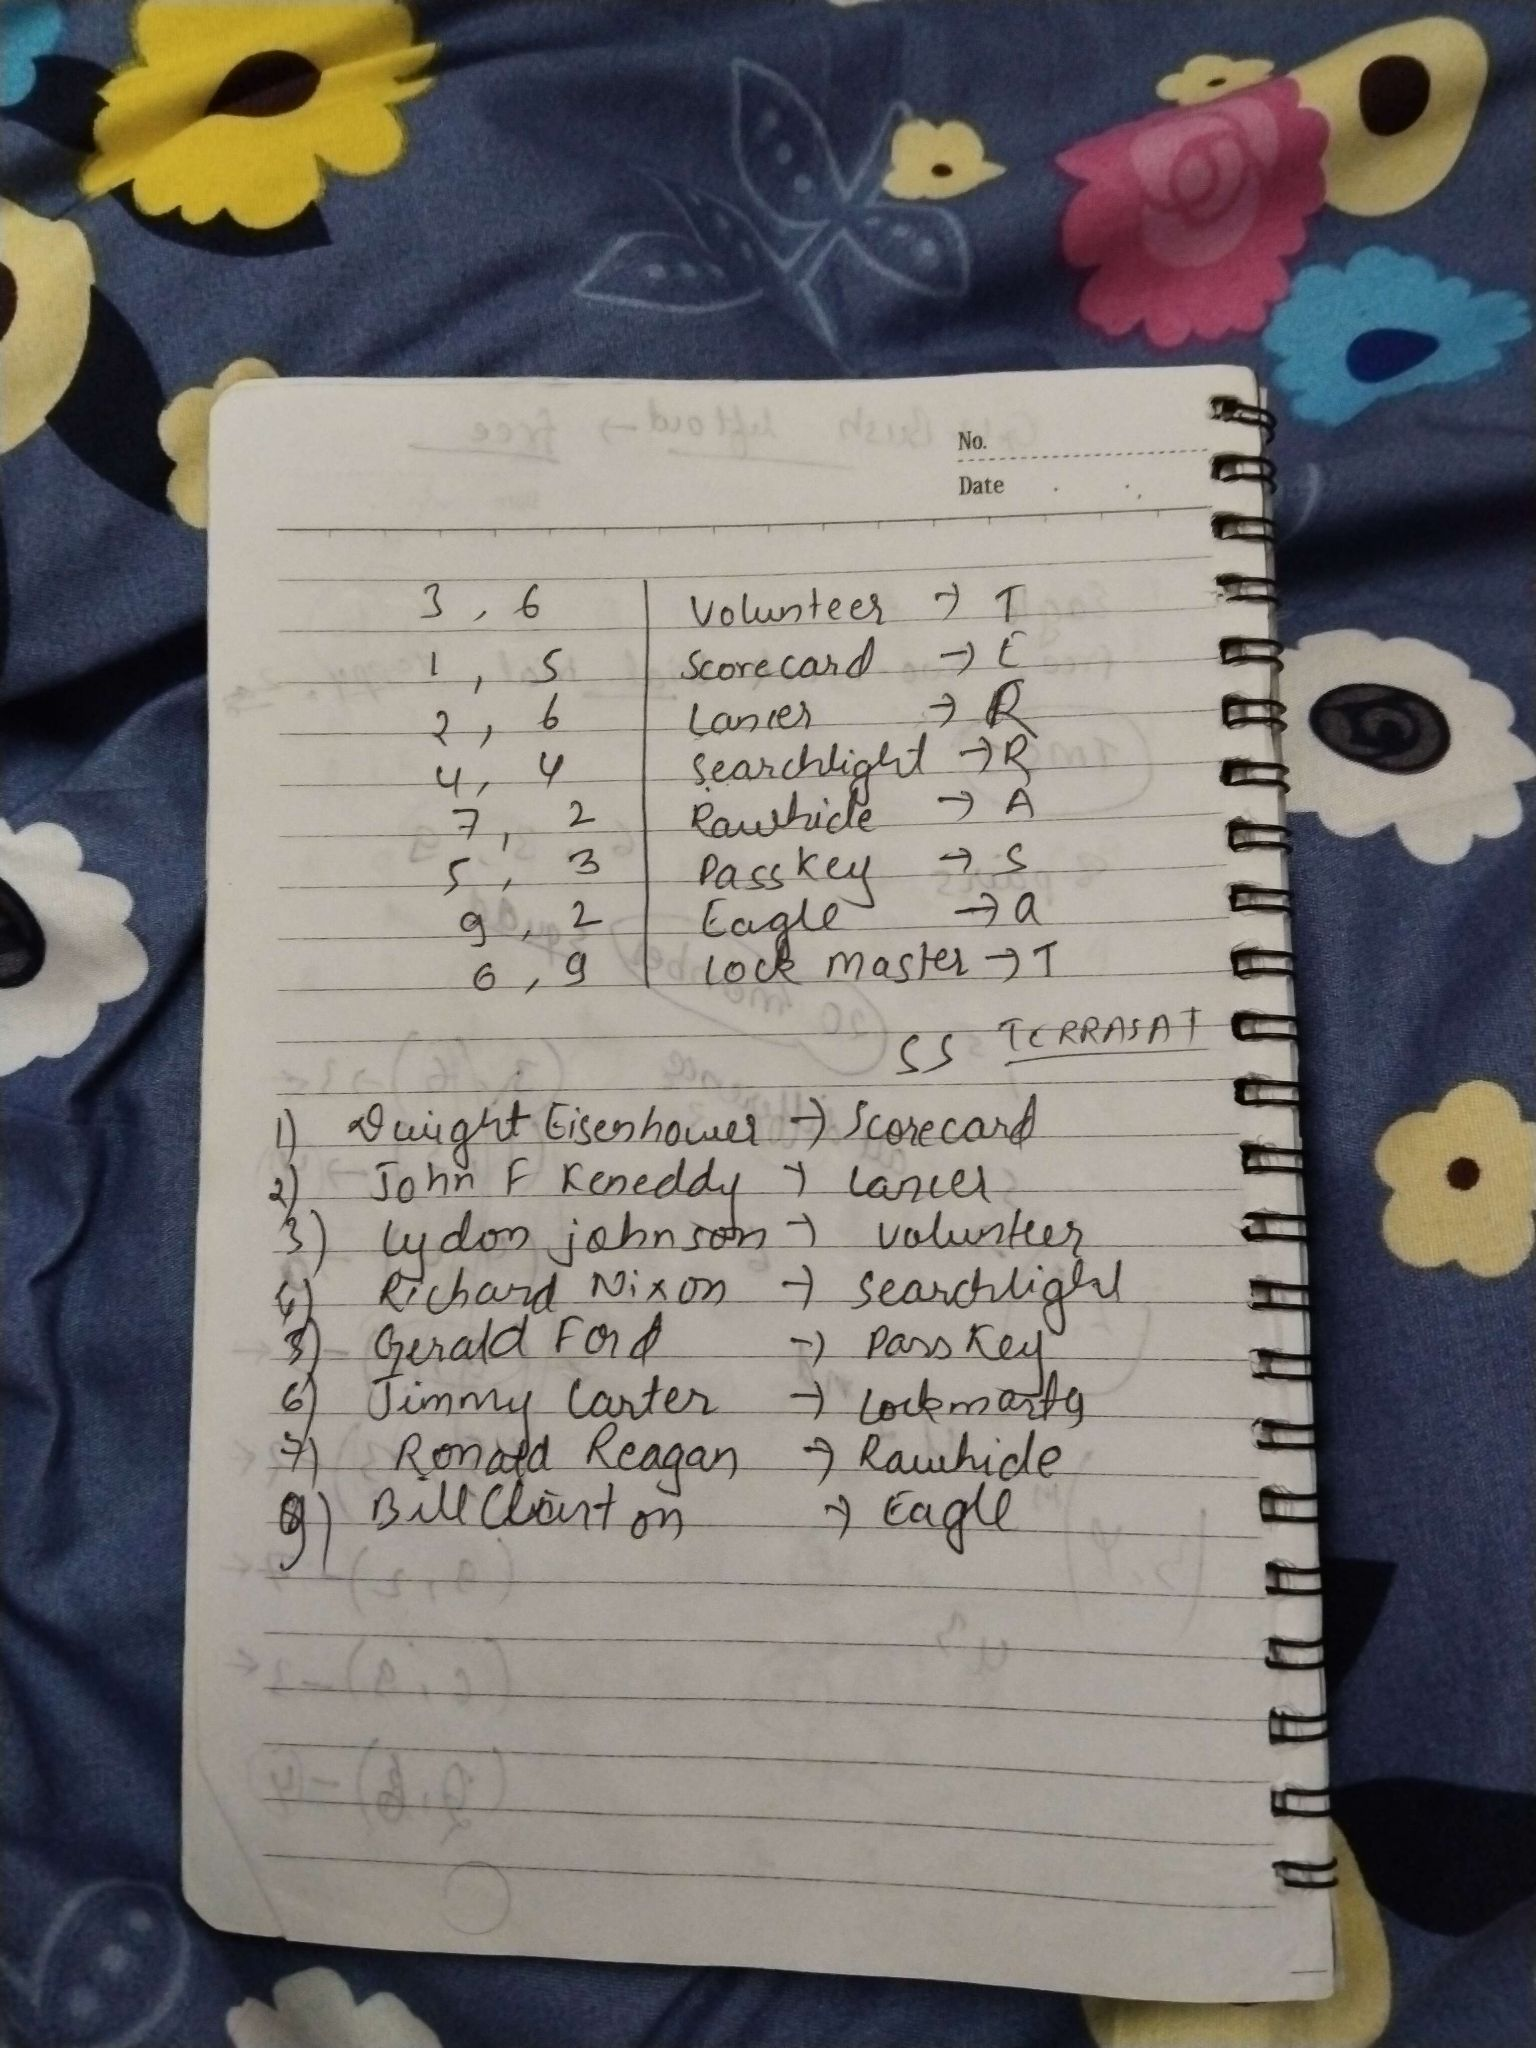
\includegraphics[width=\linewidth]{output/original.jpg}
            \caption{Original image}
        \end{minipage}
        \hspace{3cm}
        \begin{minipage}[b]{0.30\linewidth}
            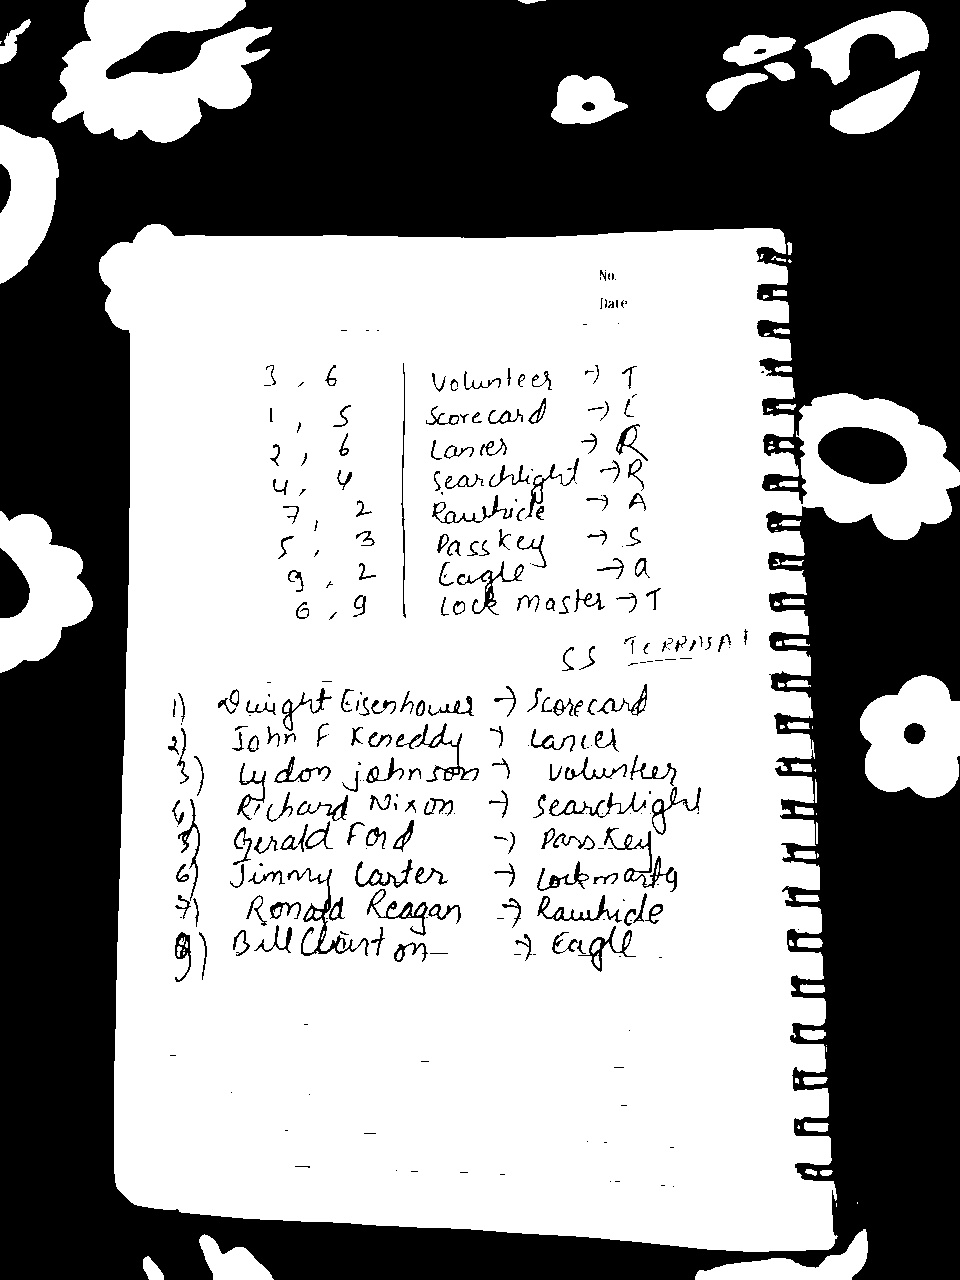
\includegraphics[width=\linewidth]{output/thresholded.jpg}
            \caption{Threshold Image}
        \end{minipage}
        
    \end{figure}
    \begin{figure}[h]
        \centering
        \begin{minipage}[b]{0.30\linewidth}
            
\includegraphics[width=\linewidth]{output/closed.jpg}
            \caption{Closed Image}
        \end{minipage}
        \hspace{3cm}
        \begin{minipage}[b]{0.30\linewidth}
            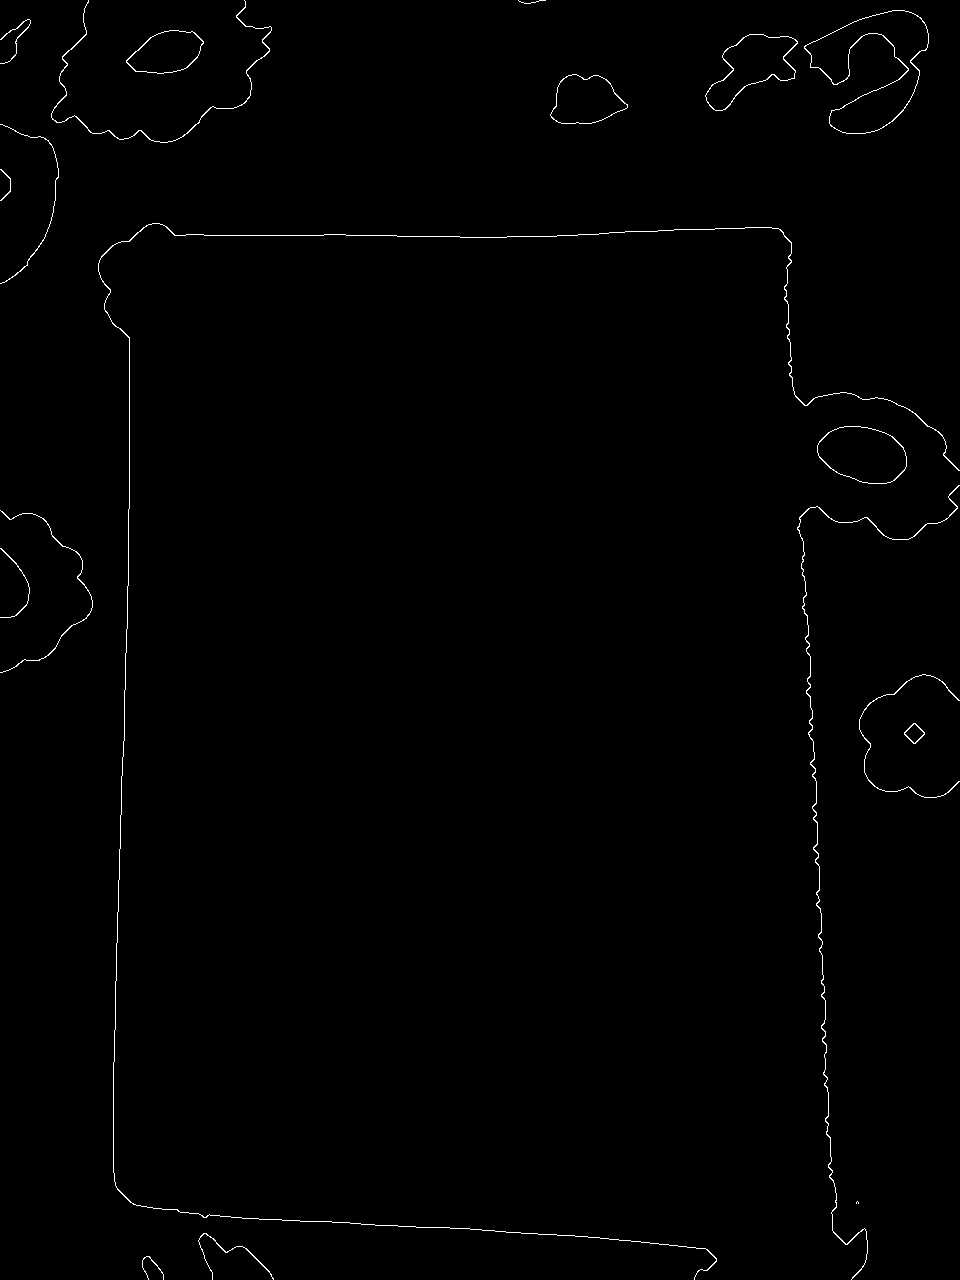
\includegraphics[width=\linewidth]{output/edges.jpg}
            \caption{Canny Edge}
        \end{minipage}
        
    \end{figure}
    \begin{figure}[h!]
        \centering
        \begin{minipage}[b]{0.30\linewidth}
            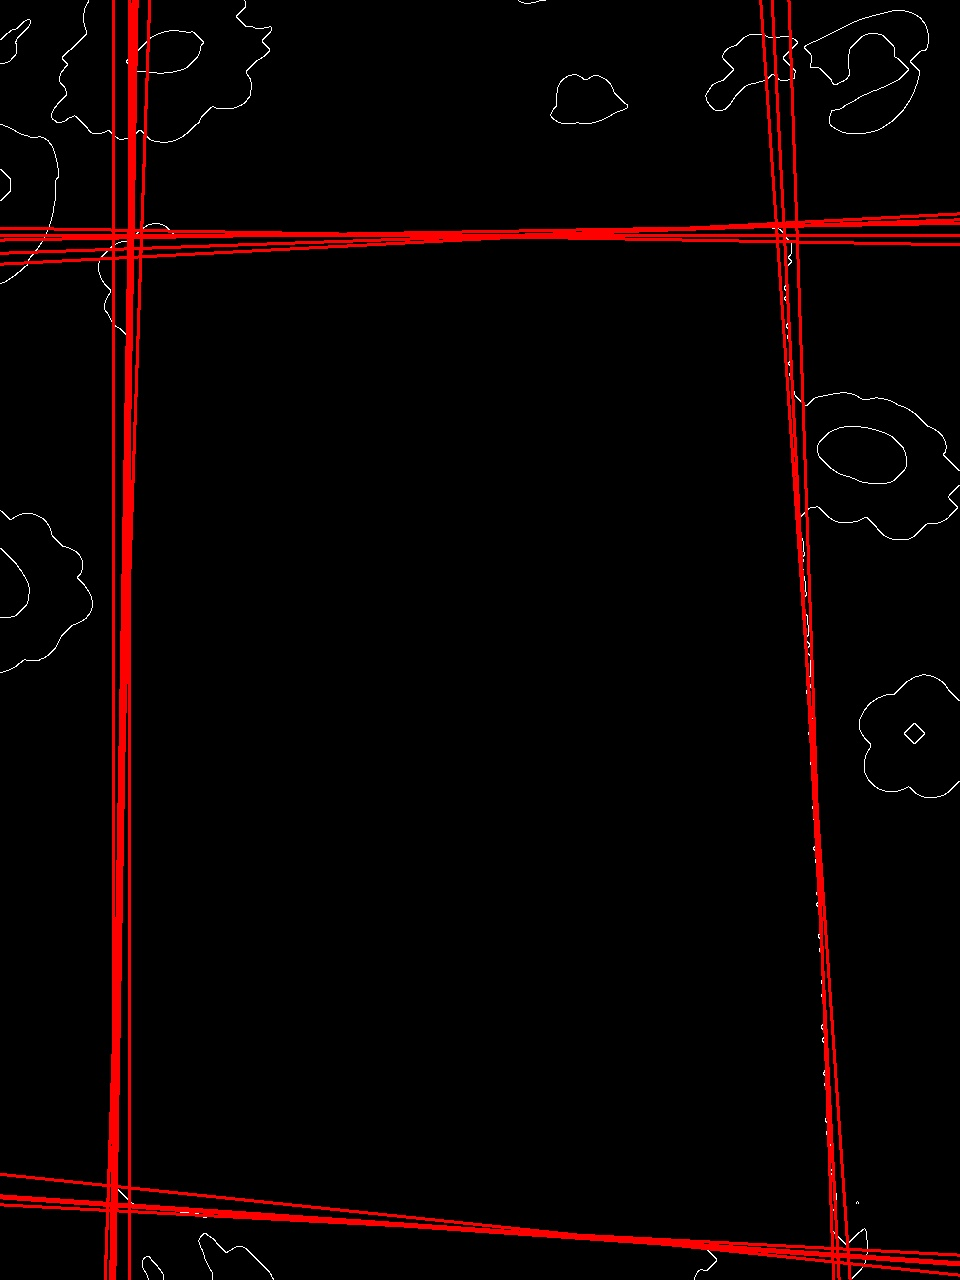
\includegraphics[width=\linewidth]{output/hough_line.jpg}
            \caption{Hough Line Image}
        \end{minipage}
        \hspace{3cm}
        \begin{minipage}[b]{0.30\linewidth}
            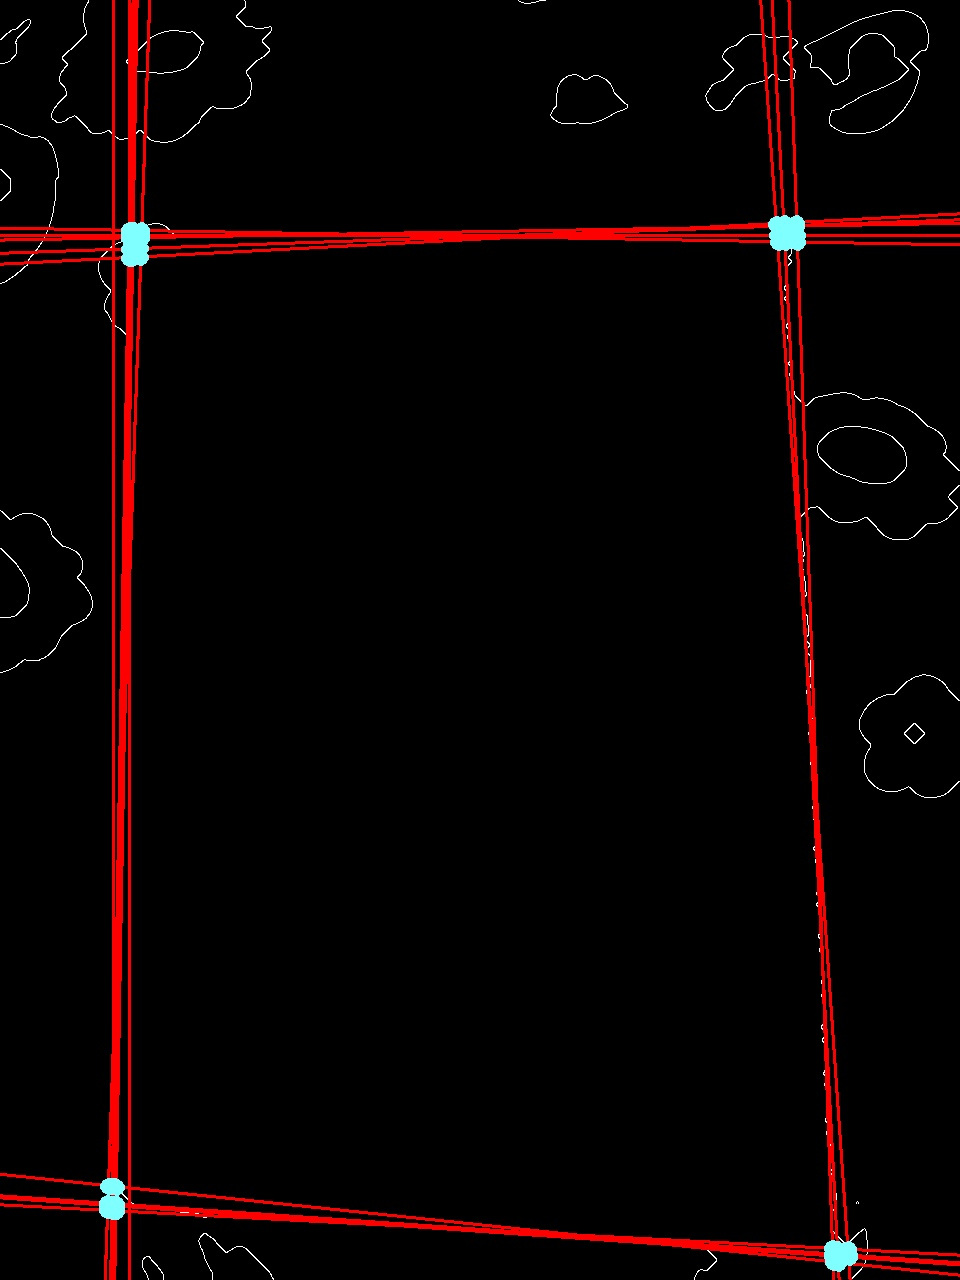
\includegraphics[width=\linewidth]{output/intersection_point_output.jpg}
            \caption{Intersection Point Image}
        \end{minipage}
        
    \end{figure}
    
    \begin{figure}[h]
        \centering
        \begin{minipage}[b]{0.30\linewidth}
            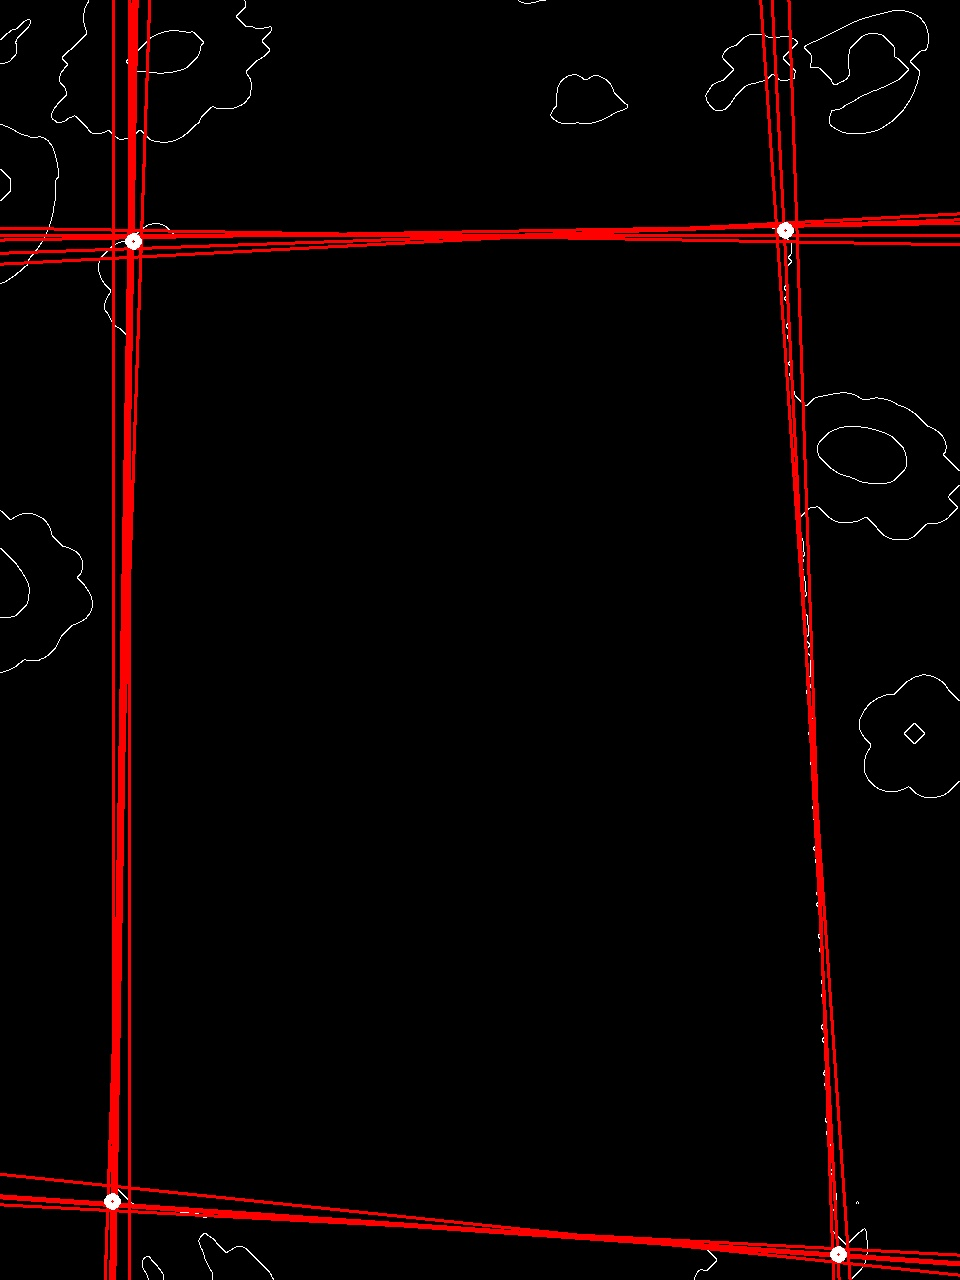
\includegraphics[width=\linewidth]{output/grouped.jpg}
            \caption{K-means Clustering Image}
        \end{minipage}
        \hspace{3cm}
        \begin{minipage}[b]{0.30\linewidth}
            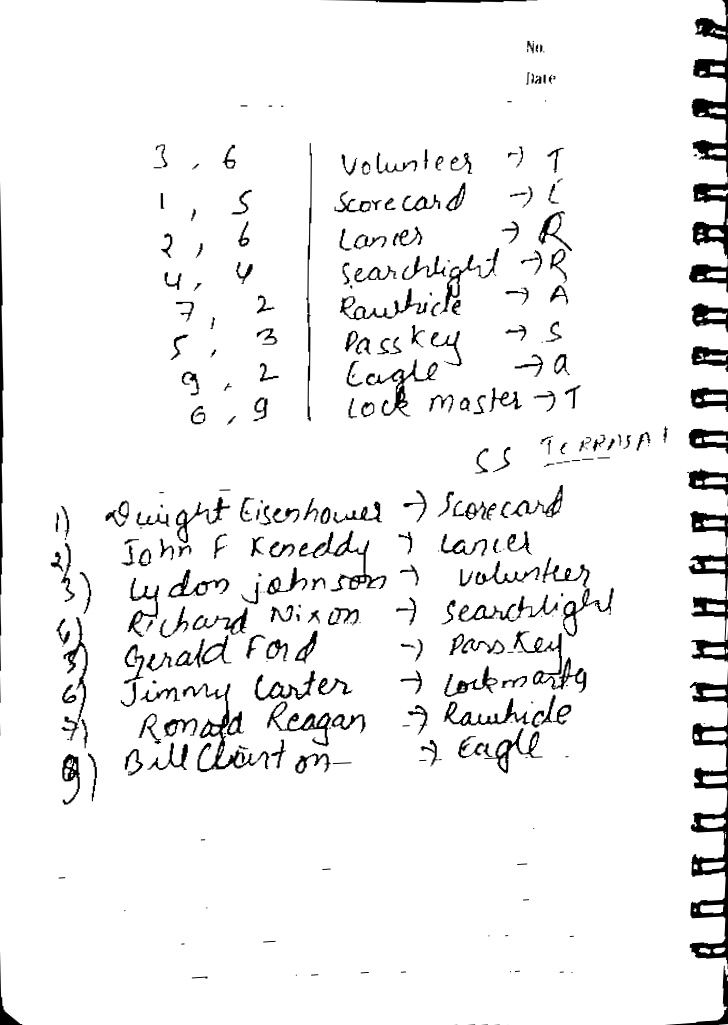
\includegraphics[width=\linewidth]{output/output.jpg}
            \caption{Preprocessing Output Image}
        \end{minipage}
        
    \end{figure}
    \newpage
\newpage
    \item Mobile App: The Mobile app for SnapTag has been developed using Flutter.
    \begin{figure}[h!]
        \centering
        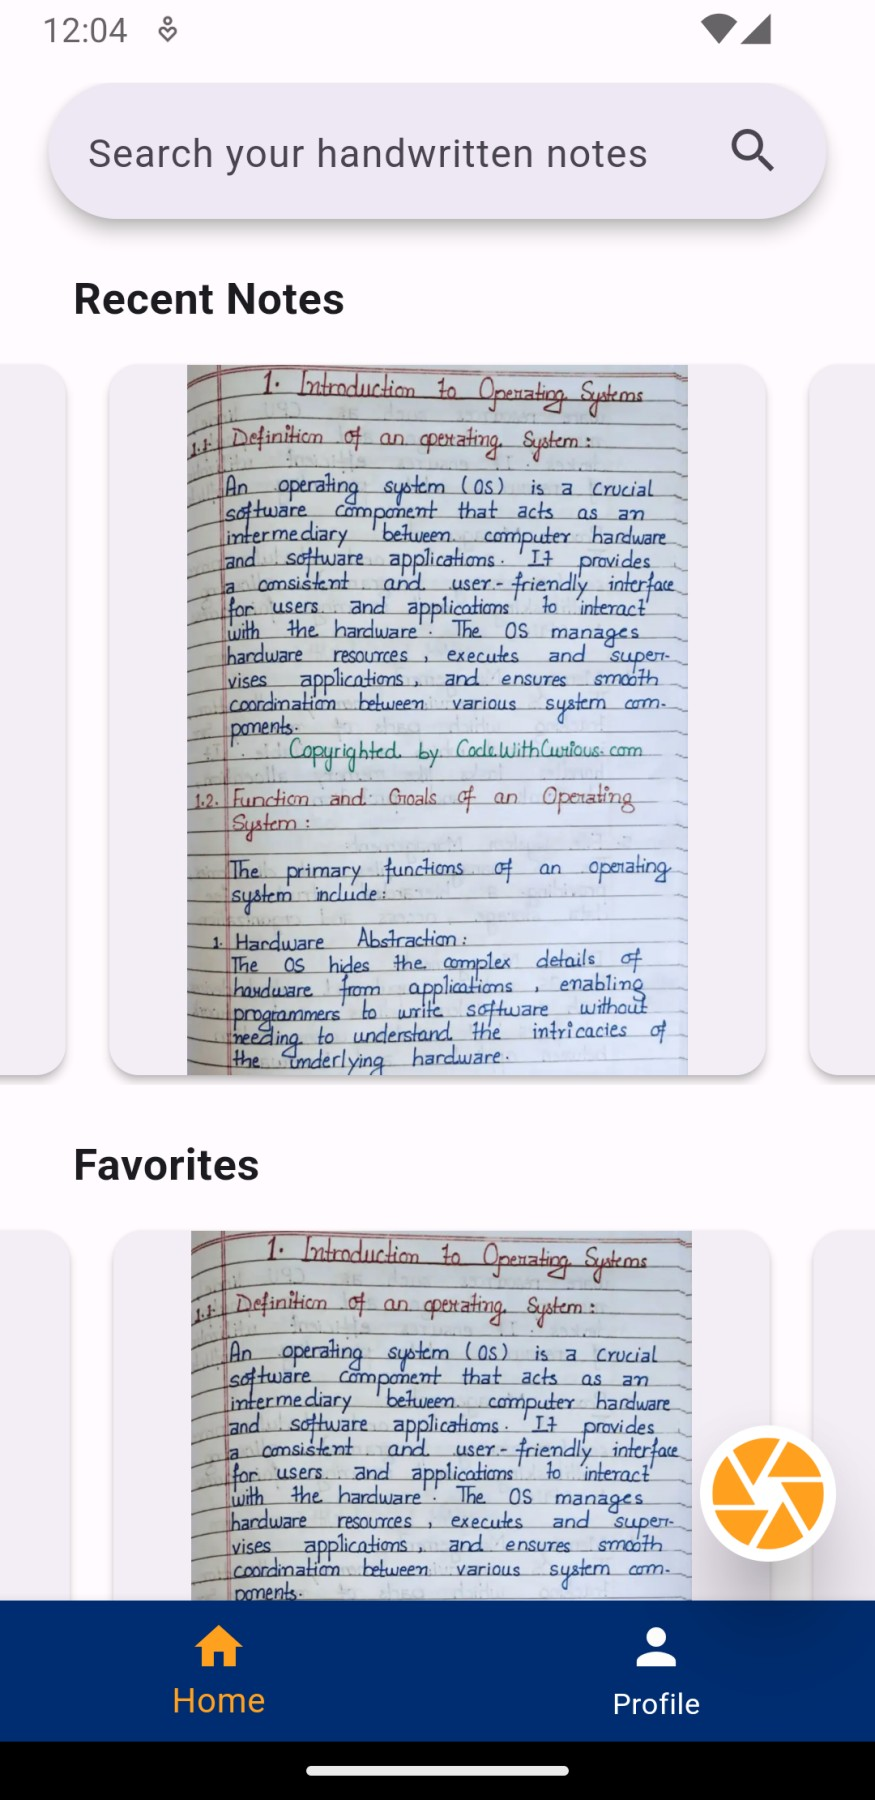
\includegraphics[scale=0.3]{output/home.jpg}
        \caption{Homepage}
        % \label{fig:segmented_image}
    \end{figure}
    \begin{figure}[h!]
        \centering
        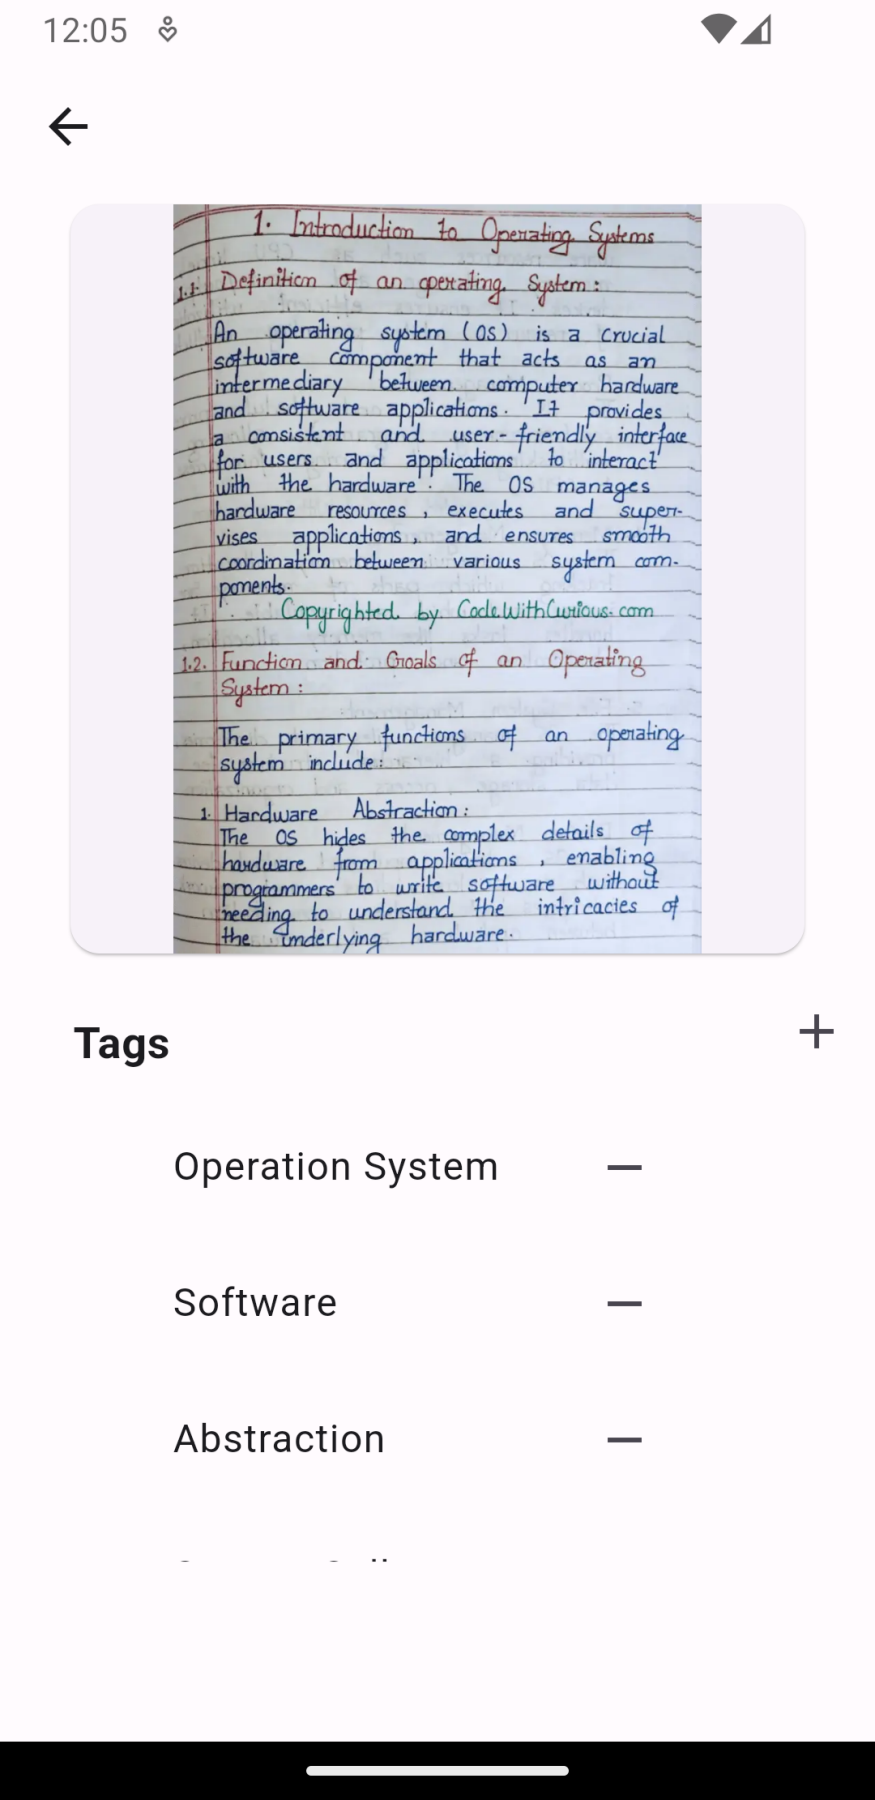
\includegraphics[scale=0.3]{output/add.png}
        \caption{Image Capturing }
        % \label{fig:segmented_image}
    \end{figure}
\end{enumerate}
\newpage
\section{Work Remaining}
\begin{enumerate}
    \item Segmentation: Till now, Line Segmentation has been done which still needs some improvements. After that, our immediate work will be segmentation words and characters. The following is the result produced using traditional Contour-Based Segmentation for lines.
    \item Model Training: The efficiency of the trained model is 82\% and we are working on improving the efficiency.
\end{enumerate}
%\section{Schedule}

%\begin{figure}[ht]
 %   \centering
  %  \includegraphics[scale=0.5]{photo/ganttchart.png}
   % \caption{Gantt Chart}
    %\label{fig:my_label}
%\end{figure}



%Reference
\renewcommand\bibname{REFERENCES} % Change heading to References
\bibliographystyle{IEEEtran} % to use IEEE Format for referencing
\addcontentsline{toc}{chapter}{References} % to add references in TOC
\bibliography{library} % specify the .bib file containing reference information 

%Comment this Chapter if you do not need to include Appendix.

%\addcontentsline{toc}{chapter}{Appendix}

\end{figure}

\end{document}
